
\front

\linespread{1.5}                        %comando per impostare l'interlinea
\pagestyle{empty}

\begin{center}
\par
\vspace{6pt}
%\begin{tabular}{p{5cm}p{5cm}}

\includegraphics[width=.16\textwidth]{../Pictures/Front/logo.png} \hspace{0.5\textwidth}
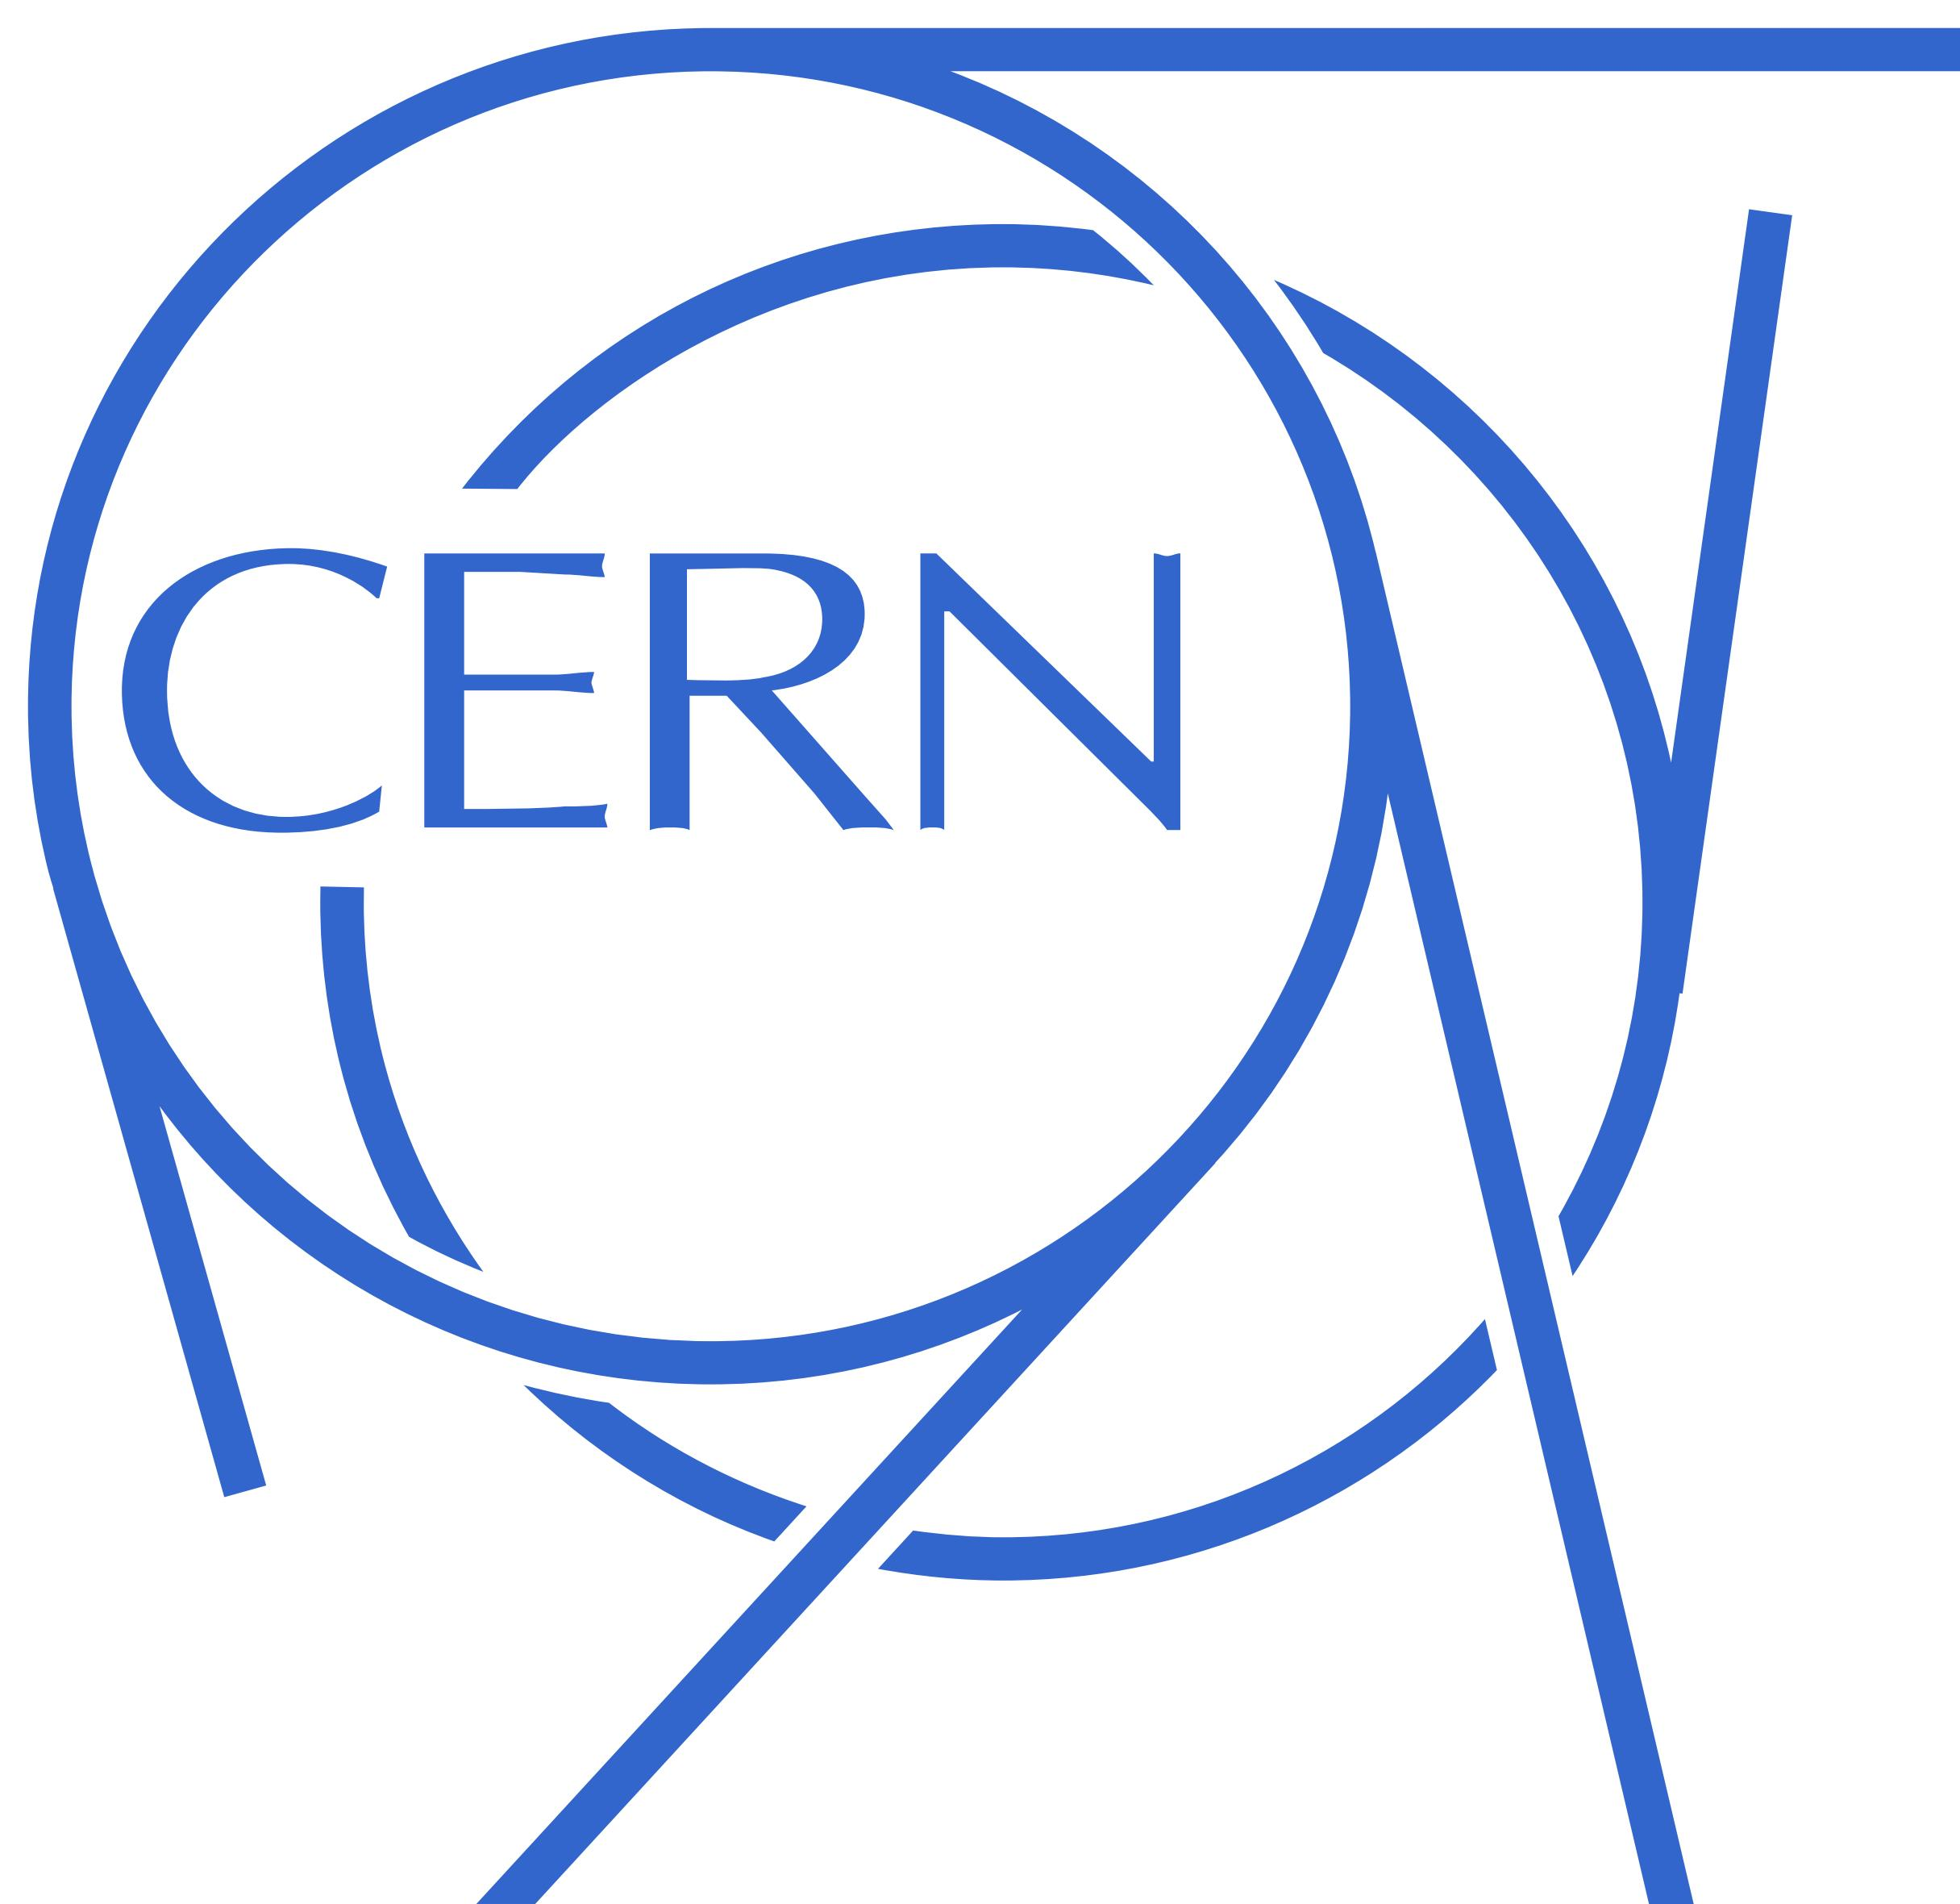
\includegraphics[width=.16\textwidth]{../Pictures/Front/cern_logo.jpg}\\
%\end{tabular}
\par
\vspace{10pt}
\hrule 
\par
\vspace{18pt}
\par
\begin{large}\textbf{Ph.D. thesis}\\
\par
\vspace{2pt}
\par
December 2014 \\ 
\par
\vspace{8pt}
\par
\end{large} 
\begin{Large}
{\bf Corso di Dottorato in Fisica e Astronomia - Ciclo XXVI}\\
\vspace{-5pt}
Dipartimento di Fisica G.Occhialini\\
\vspace{-10pt}
Universit\`a degli Studi di Milano-Bicocca\\
\vspace{-10pt}
%y\\
%\vspace{-10pt}
%Institut de F\'isica d'Altes Energies\\
\end{Large}
\vspace{80pt}
{\huge \bfseries Study of time profiles} \\
\vspace{6pt}
{\huge \bfseries of heavy scintillating crystals} \\ 
\vspace{6pt}
%{\huge \bfseries at High Luminosity LHC}\\
%\vspace{6pt}
%{\huge \bfseries }
\vspace{80pt} 
\centering
\begin{tabular}{p{10cm}p{1rcm}}
\large Doctoral Student &  \\
\Large \bfseries Nicolas Di Vara & \\
 & \\
 & \\
 & \large Tutor \\
 &\Large \bfseries Prof. Marco Paganoni\\
 &\large Universit\`a degli Studi di Milano-Bicocca\\
 &\large Dipartimento di Fisica G.Occhialini\\
 %& \\
 %& \\
 %& \large External Supervisor \\
 %&\Large \bfseries Dr. Etiennette Auffray\\
 %&\large CERN -- PH-CMX\\
 %& \\
 %& \\
\end{tabular}
\vspace{10pt} \\
\hrule \vspace{6pt}
\large 

\begin{textblock}{1}(11.5,13.5)

\includegraphics[scale=0.7]{../Pictures/Front/Logo_Marie-Curie}
\end{textblock}
\begin{textblock}{1}(3,13.5)

\includegraphics[scale=0.3]{../Pictures/Front/Entervision}
\end{textblock}
\end{center}

